OpLev (Optical Lever) は, 反射面の角度変位を測定するために使用され, 光源, 鏡, ビーム位置検出装置から構成される. また, KAGRAでは, OpLevで使用するビームはL方向の変位を測定するためにも使用することができる. これは, 凸レンズの後ろにあるビームの位置を感知することで行われる. 一般にOpLeVとは装置全体の中で角度を感知する部分を指すが, KAGRAではL・P・Yの3つの変位を感知する装置全体をOpLevと呼ぶ. \\
\quad 本論文の主な対象である低温懸架装置ではOpLevによって絶対角度変位, 絶対水平変位を測定している. 以下ではOpLevを用いた鏡のL, P, Yの変位の測定原理を記した後, KAGRAの低温懸架装置におけるOpLevの構成について述べる. 
\section{OpLevを用いた鏡の変位の測定原理}
\label{secB.1}
最も単純なのは図\ref{figB.1}に示したように, 鏡が$\theta$回転した場合である. このとき, 入射面に沿ったビーム位置$x_1$は角度変位$\theta$を用いて
\begin{equation}
x_1=(2r)\theta,
\end{equation}
と書ける. ここで, $r$はOpLevのアーム長(反射面と受光面の距離)である. \\
\quad また, 図\ref{figB.2}に示したようにビームが入射角$\alpha$を持つ場合, 鏡のL方向の変位を測定することができる. このときのビーム変位は
\begin{equation}
x_1=(2r)\theta+(2\sin\alpha)x_L,
\label{eqB.2}
\end{equation}
となる. ここで, $x_L$は鏡のL方向の変位である. この式は, 角度変位とL方向の変位がカップルしていることを示す. \\
\quad また直前のカップリングを分離するために凸レンズを挿入することで, そのカップリングを分離することができる. 図\ref{figB.3}に示すように焦点距離$f$の凸レンズの後方のある距離dでのビーム変位$x_2$を測定する第2のセンサーを持つOpLevがある. この場合, 光線行列を用いてビーム変位$x_2$を求める. 
\begin{equation}
\begin{pmatrix}
x_2\\
\theta^{\prime}
\end{pmatrix}
=\begin{pmatrix}
1&d\\
0&1
\end{pmatrix}
\begin{pmatrix}
1&0\\
-1/f&1
\end{pmatrix}
\begin{pmatrix}
1&r_{\rm lens}\\
0&1
\end{pmatrix}
\begin{pmatrix}
(2\sin\alpha)x_L\\
2\theta
\end{pmatrix}.
\end{equation}
ここで, $r_{\rm lens}$は反射面とレンズの距離である. これより
\begin{equation}
x_2=(2\sin\alpha)\left(1-\frac{d}{f}\right)x_L+2\left[\left(1-\frac{d}{f}\right)r_{\rm l}+d\right]\theta.
\label{eqB.4}
\end{equation}
\clearpage
\begin{figure}[H]
\begin{center}
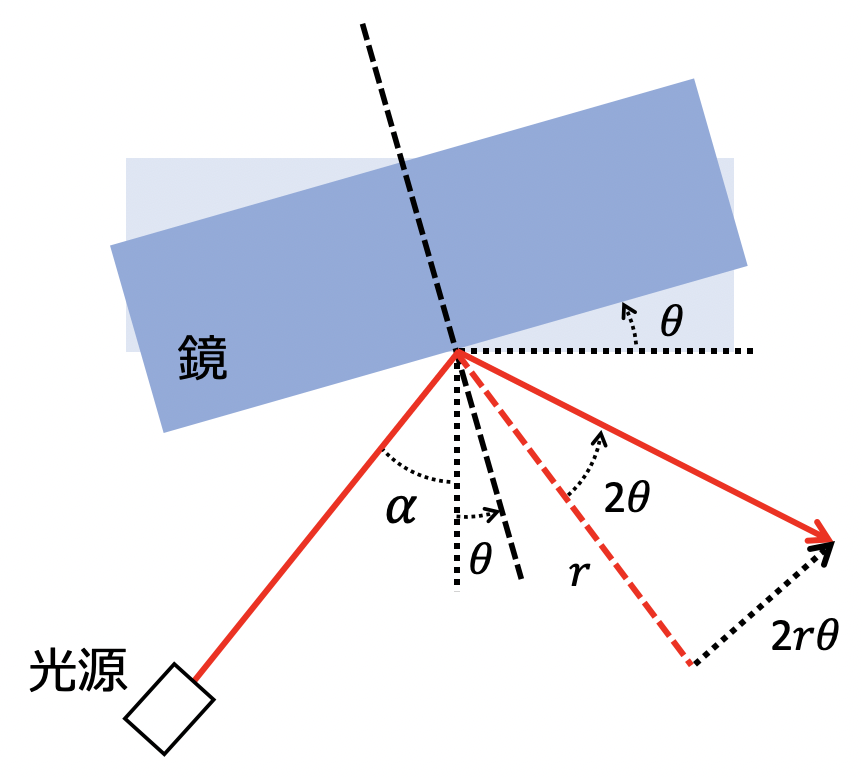
\includegraphics[width=80mm]{figB_1.png} 
\caption[鏡の回転に対するOpLev光のずれ]{鏡の回転に対するOpLev光のずれ. 鏡の回転によってOpLevのビームがずれる. 赤い点線が元の光軸を表しており, 実線は鏡が回転した時の光軸を示す. }
\label{figB.1}
\end{center}
\end{figure}
\begin{figure}[H]
\begin{center}
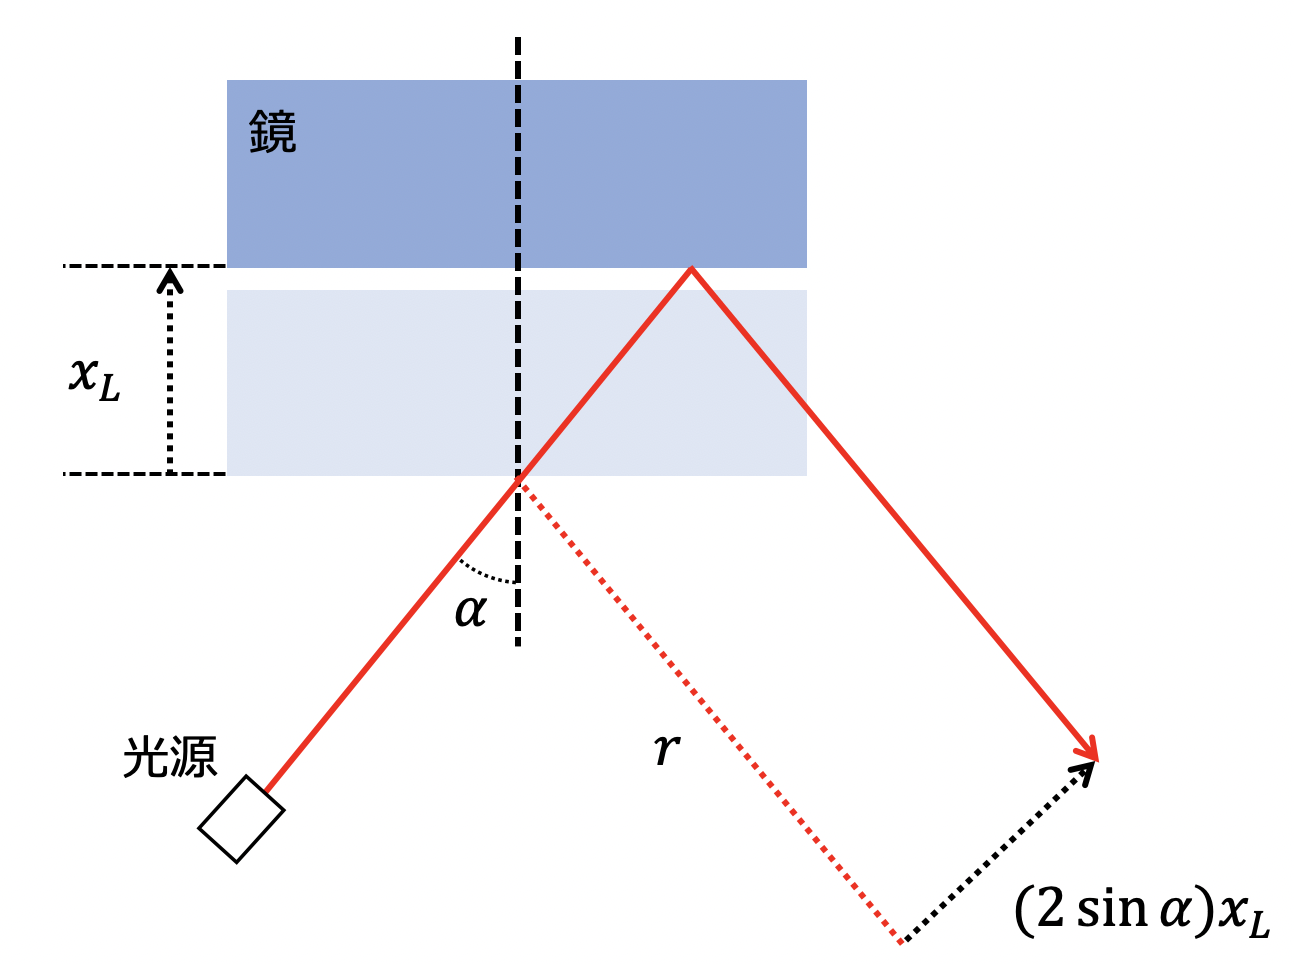
\includegraphics[width=90mm]{figB_2.png} 
\caption[鏡のL方向のずれに対するOpLev光のずれ]{鏡のL方向のずれに対するOpLev光のずれ. 赤い点線が元の光軸を表しており, 実線は鏡がL方向に移動した時の光軸を示す. }
\label{figB.2}
\end{center}
\end{figure}
\begin{figure}[H]
\begin{center}
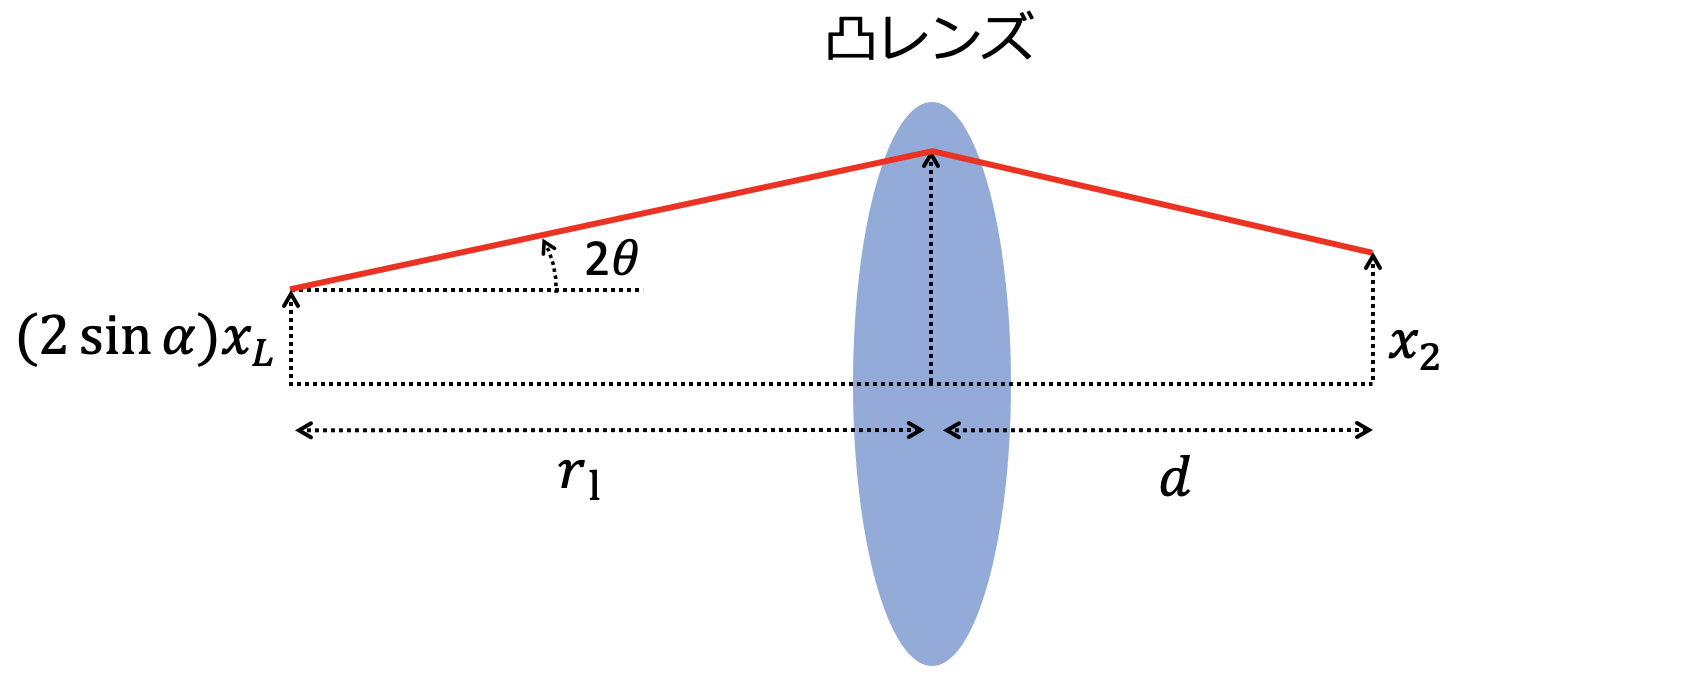
\includegraphics[width=120mm]{figB_3.png} 
\caption[レンズの後ろにあるビーム位置を感知する第2のビーム変位センサ]{レンズの後ろにあるビーム位置を感知する第2のビーム変位センサ}
\label{figB.3}
\end{center}
\end{figure}
\clearpage
\noindent
また, センサの位置を
\begin{equation}
d=\frac{r_{\rm l}f}{r_{\rm l}-f},
\label{eqB.5}
\end{equation}
と設定することによって式(\ref{eqB.4})の右辺第2項, つまり角度のカップリングを0にすることができる. これにより, 第2のビーム変位センサはL方向(length sensing)のセンサとなる. \\
\quad 式(\ref{eqB.5})が成り立つ場合, length sensing センサで読み取れるビーム変位は
\begin{equation}
x_2=\left(\frac{-2f\sin\alpha}{r_{\rm l}-f}\right)x_L,
\label{eqB.6}
\end{equation}
となる. ここで, 式(\ref{eqB.2})を式(\ref{eqB.6})に代入すると, 
\begin{equation}
\begin{pmatrix}
x_L\\
\theta
\end{pmatrix}
=
\begin{pmatrix}
2\sin\alpha&2r\\
\frac{-2f\sin\alpha}{r_{\rm l}-f}&0
\end{pmatrix}
^{-1}
\begin{pmatrix}
x_1\\
x_2
\end{pmatrix},
\end{equation}
のようにセンシング行列が得られるので, これを用いてセンサの対角化が行われる. 

\section{KAGRAの低温懸架系におけるOpLeV}
KAGRAではtilt sensing OpLev(\ref{secB.1}に最も単純なものと記したもの)とlength sensing OpLev(\ref{secB.1}に第2のビーム変位センサとして記したもの)の2種類が用いられている. これらは共に水平方向, 垂直方向のビームスポットの変位を見ることができるので, それを($x_{\rm tilt},y_{\rm tilt}$), ($x_{\rm len},y_{\rm len}$)と書く. \\
また, KAGRAでは反射光を検知する光検出器としてQPD (Quadrant PhotoDiode)を用いている. ここで, QPDとは4つに分割されたPDであり, それぞれの領域に入射した光の強度を測定している. KAGRAでは各領域のカウント数と全体のカウント数からQPD上の距離を算出している(図\ref{figB.4}). このQPDはビームに対して垂直に設置されているので, QPDで検出したビームスポット位置の変位は一般的にはグローバルな水平, 垂直方向に対して平行ではない. 
\begin{figure}[H]
\begin{center}
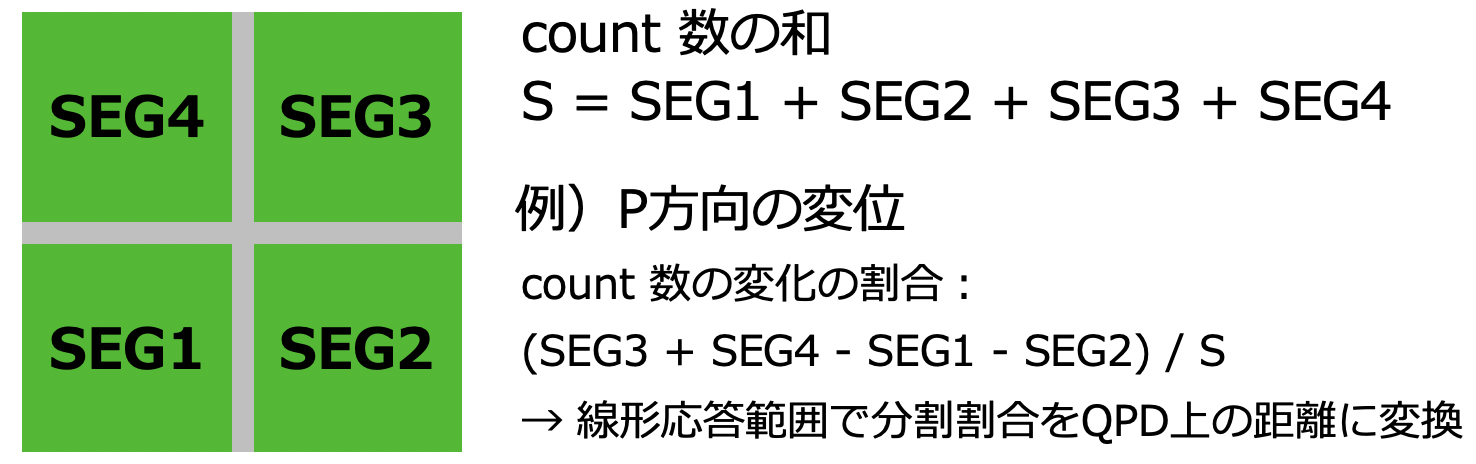
\includegraphics[width=150mm]{figB_4.png} 
\caption[QPD]{QPDの図. 各領域のカウント数からQPD上の距離を算出している. }
\label{figB.4}
\end{center}
\end{figure}
ここで, 特に関心があるのは鏡の変位のうち, L方向:$x_L$, P方向:$\theta_P$, Y方向:$\theta_Y$であるから$\bm{x}=(x_{\rm tilt},y_{\rm tilt},x_{\rm lim},y_{\rm lim})^{\rm T}$を鏡の動き$(x_L,\theta_P,\theta_Y)^{\rm T}$に対応させる行列を求めればよい. \\
\quad OpLevの腕を任意のベクトル$\bm{r}=r_x\hat{x}+r_y\hat{y}+r_z\hat{z}$で表す. なお, $\hat{x}$は鏡のT方向, $\hat{y}$は鏡のV方向, $\hat{z}$は鏡のL方向である. また, 簡単のためB.2節ではビームのミスセンタリングはないものとする(図\ref{figB.5},\ref{figB.6}中の$\delta_x,\,\delta_y=0$). 
\begin{figure}[H]
\begin{center}
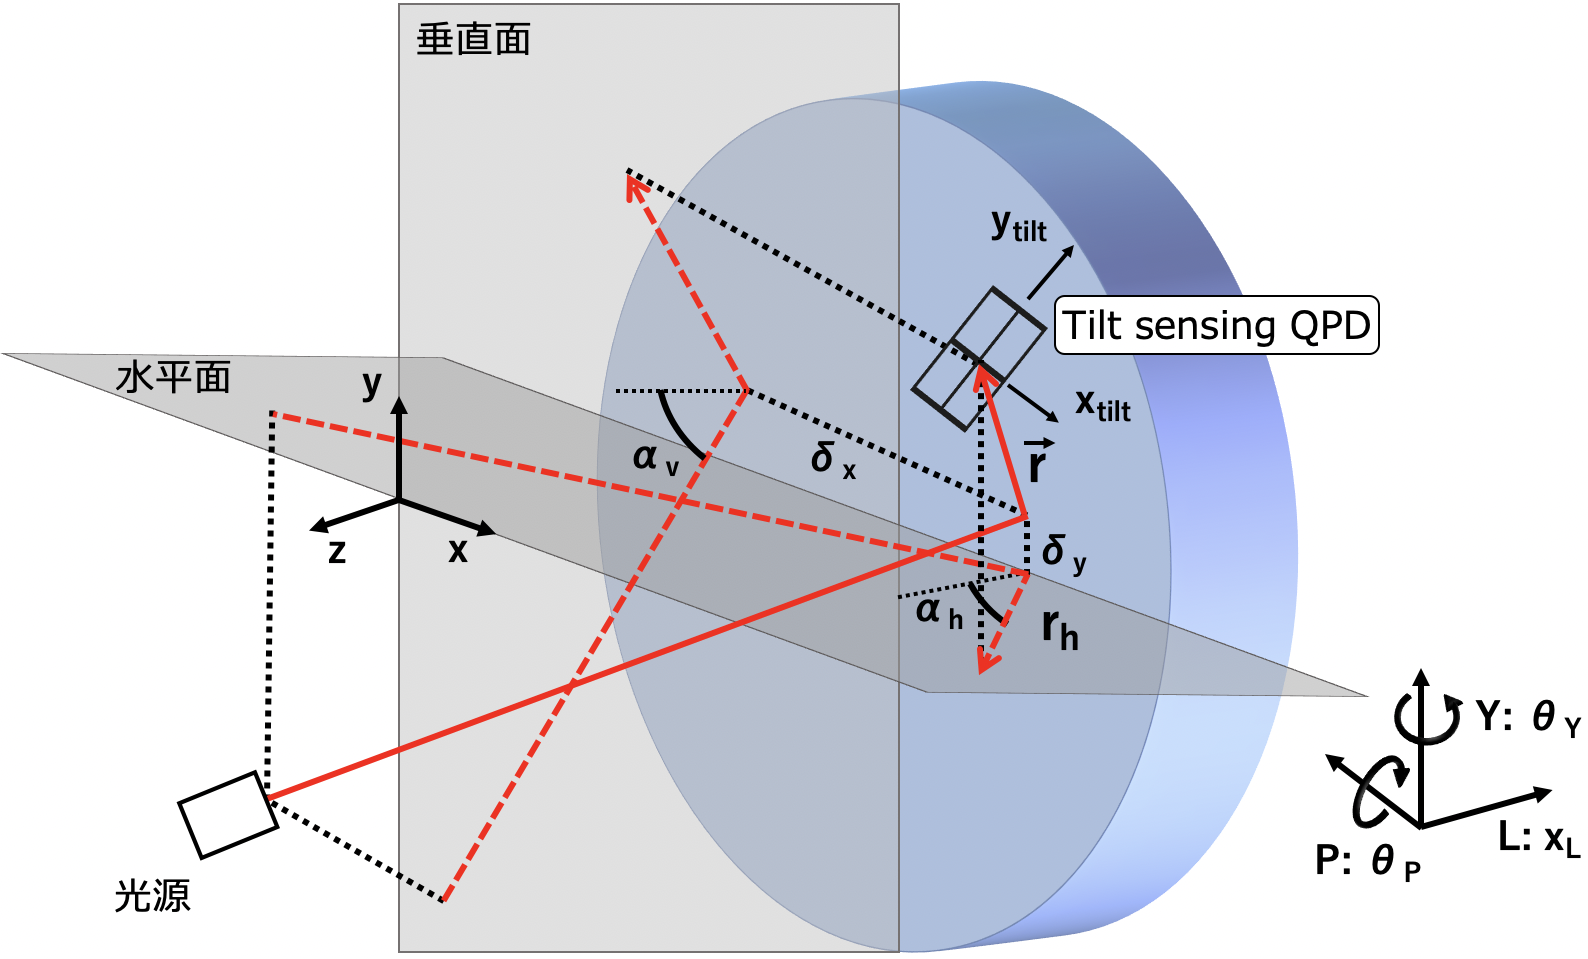
\includegraphics[width=130mm]{figB_5.png} 
\caption[KAGRAにおけるtilt-sensing OpLeVのセットアップ]{KAGRAにおけるtilt sensing OpLeVのセットアップ. 実線はビームを, 点線はその水平面・垂直面への投影である. }
\label{figB.5}
\end{center}
\end{figure}
\begin{figure}[H]
\begin{center}
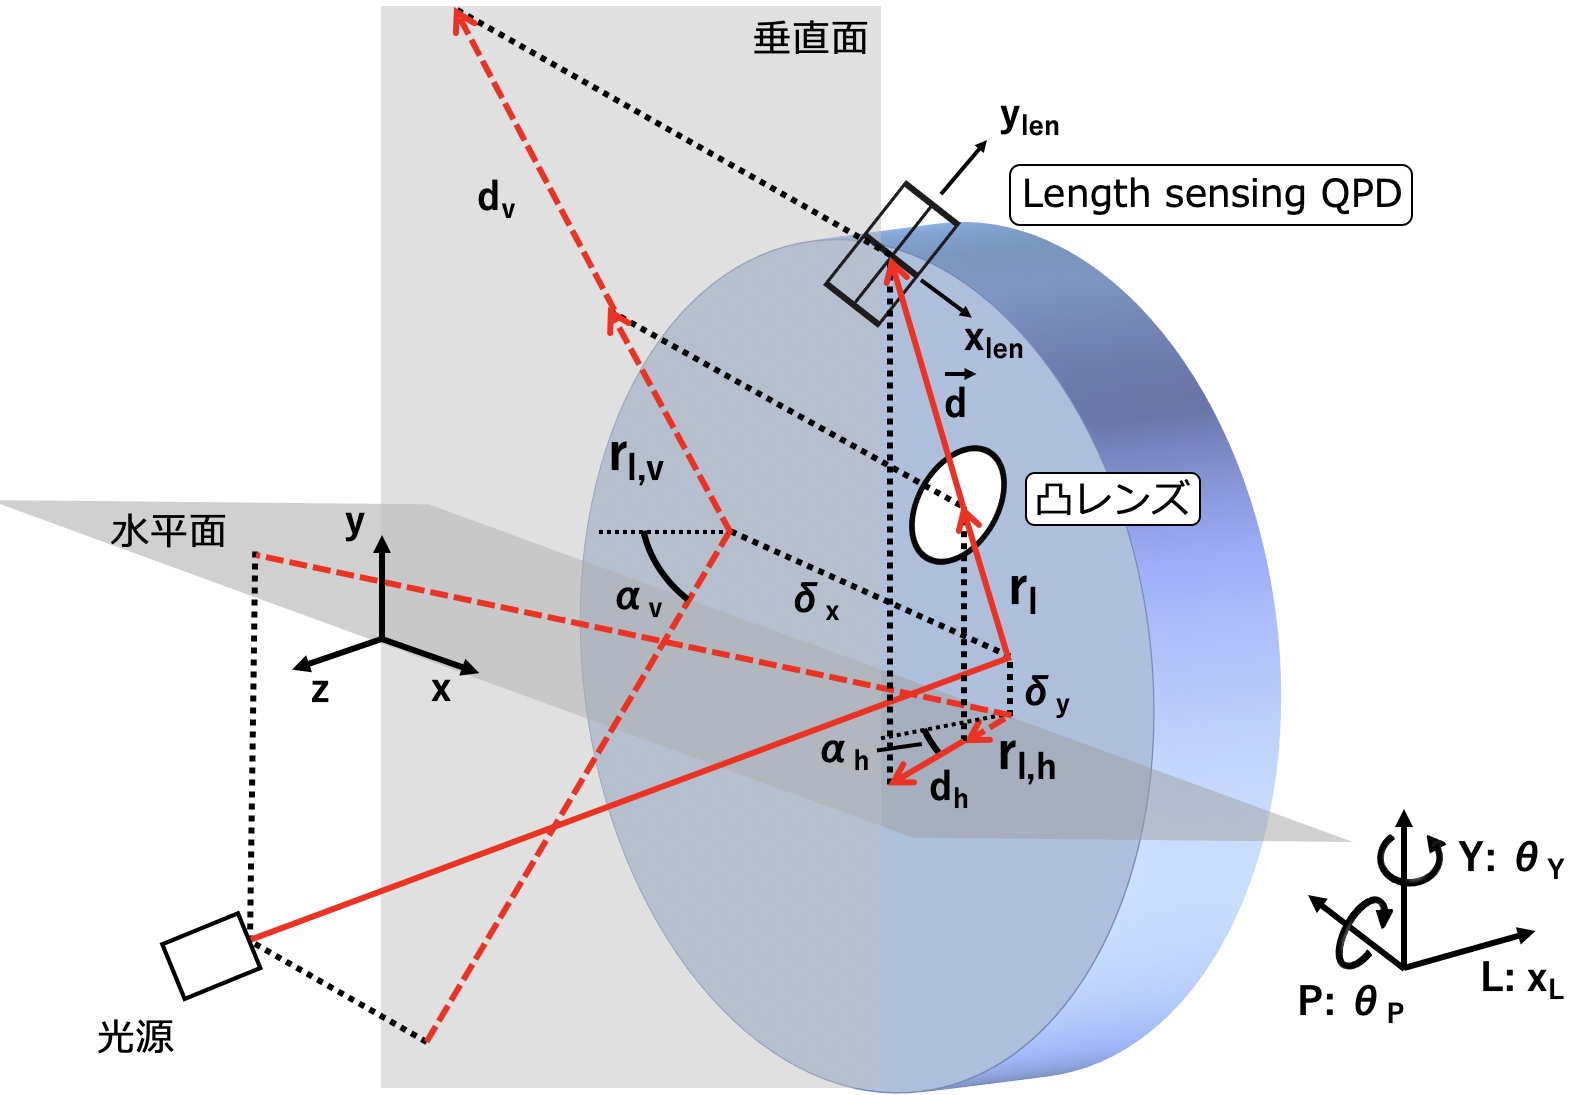
\includegraphics[width=130mm]{figB_6.png} 
\caption[KAGRAにおけるlength-sensing OpLeVのセットアップ]{KAGRAにおけるlength sensing OpLeVのセットアップ. 実線はビームを, 点線はその水平面・垂直面への投影である. tilt sensing OpLeVの場合と比べ, レンズが追加されている.}
\label{figB.6}
\end{center}
\end{figure}
tilt sensing OpLevのセットアップは図\ref{figB.5}に示す通りである. 
ビームを水平面と垂直面に投影すると, ビームの入射角は水平面では$\alpha_h$, 垂直面では$\alpha_v$となる. これよりP角を増幅するのは, レバーアームの垂直面への投影長さ$r_v$となる. 同様に, Y角を増幅するのは, レバーアームの水平面上への投影の長さ$r_h$となる. したがって$\theta_Y$と$\theta_P$の回転により, レバーアーム先端のビームスポットは水平面上で$(2r_h)\theta_Y$, 垂直面上で$(2r_v)\theta_P$だけ移動することになる. 一方, L方向のシフト$x_L$により, ビームスポットは水平面と垂直面でそれぞれ$(2\sin\alpha_h)x_L$と$(2\sin\alpha_v)x_L$だけ移動することになる. これより鏡上のビームスポットから$|\bm{r}|$離れた位置にあるtilt sensing OpLevのQPDによって測定されたビームスポットの変位は, 回転と縦方向のシフトによるものを単純に重ね合わせたもので書ける. 
\begin{equation}
x_{\rm tilt}=(2r_h)\theta_Y+(2\sin\alpha_h)x_L,
\label{eqB.8}
\end{equation}
\begin{equation}
y_{\rm tilt}=(2r_v)\theta_P+(2\sin\alpha_v)x_L.
\label{eqB.9}
\end{equation}
\quad 一方, length sensing OpLevのセットアップは図\ref{figB.6}に示す通りである(ビームは図\ref{figB.5}と同じ). ここで, 鏡から焦点距離$f$の凸レンズまでの方向を$\bm{r}_{\rm l}$と書く. 水平面へのレバーアームの射影を$r_{{\rm l},h}$とすると, length sensing OpLevのQPD上におけるビームスポット変位は光線行列を用いて
\begin{equation}
x_{\rm len}=(2\sin\alpha_h)\left(1-\frac{d_h}{f_h}\right)x_L+2\left[\left(1-\frac{d_h}{f_h}\right)r_{{\rm l},h}+d_h\right]\theta_Y,
\label{eqB.10}
\end{equation}
と書ける. ここで$d_h$はレンズとlength sensing OpLevのQPDとの水平面上の距離, $f_h$は水平面上での焦点距離である. また, 
\begin{equation}
r_{{\rm l},h}=|\bm{r}_{\rm l}|\cos\theta_h,
\label{eqB.11}
\end{equation}
となるように水平面とビームの角度$\theta_h$を導入する. さらに, レンズとlength sensing OpLevのQPDとの水平面上の距離や焦点距離についても同様に
\begin{equation}
d_h=|\bm{r}_{\rm l}|\cos\theta_h,
\label{eqB.12}
\end{equation}
\begin{equation}
f_h=f\cos\theta_h,
\label{eqB.13}
\end{equation}
と書ける. ここで式(\ref{eqB.11}), (\ref{eqB.12}), (\ref{eqB.13})を式(\ref{eqB.10})へ代入すると
\begin{equation}
x_{\rm len}=(2\sin\alpha_h)\left(1-\frac{d}{f}\right)x_L+2\cos\theta_h\left[\left(1-\frac{d}{f}\right)r_{\rm l}+d\right]\theta_Y,
\end{equation}
となるのでlength sensing OpLevのQPDは
\begin{equation}
d=\frac{r_{\rm l}f}{r_{\rm l}-f},
\label{eqB.15}
\end{equation}
に置けば良いと分かる(これは式(\ref{eqB.5})と同じである. ). 一方, 式(\ref{eqB.10})において水平面に射影した量を垂直面の場合に置き換えると, length sensing OpLevのQPD上におけるビームスポットの垂直方向の変位は
\begin{equation}
y_{\rm len}=(2\sin\alpha_v)\left(1-\frac{d_v}{f_v}\right)x_L+2\left[\left(1-\frac{d_v}{f_v}\right)r_{{\rm l},v}+d_h\right]\theta_P,
\label{eqB.16}
\end{equation}
となる. \\
\quad ここで正しく設置されたOpLevに対し, センシング行列を${\rm{\textbf{C}}}_{\rm align}$として式(\ref{eqB.8}), (\ref{eqB.9}), (\ref{eqB.10}), (\ref{eqB.16})をまとめると
\begin{equation}
\begin{pmatrix}
x_L\\
\theta_P\\
\theta_Y
\end{pmatrix}
={\rm{\textbf{C}}}_{\rm align}
\begin{pmatrix}
x_{\rm tilt}\\
y_{\rm tilt}\\
x_{\rm len}\\
y_{\rm len}
\end{pmatrix}.
\label{eqB.17}
\end{equation}
ここで
\begin{equation}
{\rm{\textbf{C}}}_{\rm align}=
\begin{pmatrix}
2\sin\alpha_h & 0 & 2r_h\\
2\sin\alpha_v & 2r_v & 0\\
2\sin\alpha_h\left(1-\frac{d_h}{f_h}\right) & 0 & 2\left[\left(1-\frac{d_h}{f_h}\right)r_{{\rm l},h}+d_h\right]\\
2\sin\alpha_v\left(1-\frac{d_v}{f_v}\right) & 2\left[\left(1-\frac{d_v}{f_v}\right)r_{{\rm l},v}+d_v\right] & 0
\end{pmatrix}^+.
\end{equation}
なお, $\left[\cdot\right]^+$は$\left[\cdot\right]$の擬似逆行列であり, $\left[\cdot\right]^+\left[\cdot\right]={\rm{\bm{I}}}$である. \\
入射面が水平 (HOR) 面または垂直 (VER) 面に沿っていると仮定すると, 式(\ref{eqB.17})は以下のように簡略化できる. \\\\
\noindent
\textbf{\underline{HOR OpLevの場合}}\\
$\alpha_v=0$であり, length sensing QPDの垂直方向の読み値$y_{\rm len}$は理想的には0となる. そこで, センシング行列がフルランクになるように, $y_{\rm len}$を省略できる. したがって, HOR OpLevセンシング行列は
\begin{equation}
\begin{pmatrix}
x_L\\
\theta_P\\
\theta_Y
\end{pmatrix}
=
\begin{pmatrix}
2\sin\alpha_h & 0 & 2r_h\\
0 & 2r_v & 0\\
-\frac{2f\sin\alpha_h}{r_{\rm l}-f} & 0 & 0
\end{pmatrix}^{-1}
\begin{pmatrix}
x_{\rm tilt}\\
y_{\rm tilt}\\
x_{\rm len}
\end{pmatrix},
\end{equation}
となる. ここで, length sensing QPDの位置は凸レンズから$d=d_h=\frac{r_{\rm l}f}{r_{\rm l}-f}$離れた位置にあると仮定した. なお, HOR OpLevではビームは水平面上にあるのでレバーアームは$r_h=r$であり, 垂直面への射影は$r_v=r\cos\alpha_h$である. さらに鏡からレンズまでの水平方向のアームの変位は$r_{{\rm l},h}=r_{\rm l}$となる. \\\\
\textbf{\underline{VER OpLevの場合}}\\
$\alpha_h=0$であり, length sensing QPDの垂直方向の読み値$x_{\rm len}$は理想的には0となるので, HOR OpLevの場合と同じようにセンシング行列がフルランクとなるよう$x_{\rm len}$を省略すると
\begin{equation}
\begin{pmatrix}
x_L\\
\theta_P\\
\theta_Y
\end{pmatrix}
=
\begin{pmatrix}
0 & 0 & 2r_h\\
2\sin\alpha_v & 2r_v & 0\\
-\frac{2f\sin\alpha_v}{r_{\rm l}-f} & 0 & 0
\end{pmatrix}^{-1}
\begin{pmatrix}
x_{\rm tilt}\\
y_{\rm tilt}\\
y_{\rm len}
\end{pmatrix}.
\end{equation}
ここで, 先ほどと同様に$d=d_v=\frac{r_{\rm l}f}{r_{\rm l}-f}$であり, $r_v=r$, $r_h=r\cos\alpha_v$, $r_{{\rm l},v}=r_{\rm l}$である. 